\documentclass[
  11pt,
  letterpaper,
   addpoints,
   answers
  ]{exam}

\usepackage{../exercise-preamble}

\begin{document}

\noindent
\begin{minipage}{0.47\textwidth}

\includegraphics[width=\textwidth]{../fcfm_die}
\end{minipage}
\begin{minipage}{0.53\textwidth}
\begin{center} 
\large\textbf{Conversion de la energia y sistemas Electricos} (EL3103) \\
\large\textbf{Tarea 1} \\
\normalsize Prof.~Constanza Ahumada - Rodrigo Moreno V.\\
\normalsize Prof.~Aux.~Javiera Pacheco - Erik Saez.
\normalsize Ayudantes.~Manuel Aceituno - Pamela Acuña - Alvaro Flores 
\end{center}
\end{minipage}

\vspace{0.5cm}
\noindent
\vspace{.85cm}
\hrule
\textbf{Indicacciones: La tarea se puede realizar en grupos de 3 personas . Debe ser entregada el dia viernes 13 de Septiembre , no se aceptan atrasos, el formato debera ser tipo informe.}
\hrule
\noindent
\vspace{.85cm}
\begin{questions}
    %%%%%%%%%%%%%%%%%%%%%%%%%%%
    \question Considere un cartel de permeabilidad magnética infinita y masa bien distribuida de 0 1 [kg] levitando debajo de un circuito magnético fijo que posee dos núcleos magnéticos semicirculares de iguales dimensiones, con la disposición que se muestra en la figura, tienen radio interno 6 [cm], radio externo 8 [cm] y profundidad de 2 [cm]. Permeabilidad relativa $µ_{r} =2$ para el núcleo asociado a la primera bobina y $µ_{r}=3$ para la segunda.
    \begin{figure}[h!]
        \centering
        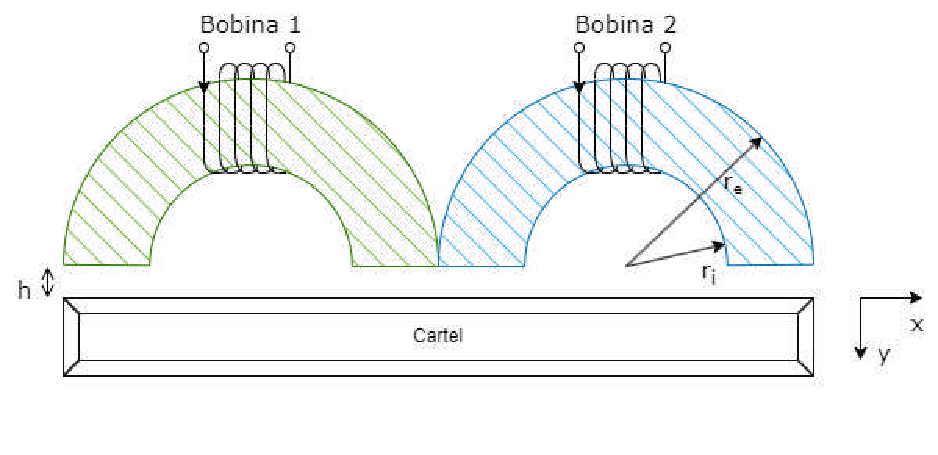
\includegraphics[width=0.5\textwidth]{Tarea_1_1}
    \end{figure}
    \begin{enumerate}[label=\alph*)]
        \item \textbf{(1.5 Puntos)} Calcule el circuito equivalente del sistema, calcule las reluctancias de los elementos presentes y la inductancia propia de cada bobina.
        \item \textbf{(2 Puntos)} Encuentre la relación que deben cumplir las fuerzas magnetomotrices para que el cartel no quede desnivelado
        \item \textbf{(2 Puntos)} Considerando que ambas bobinas tienen 200 vueltas, calcule la corriente necesaria en cada bobina para que el cartel quede a 3mm de los núcleos (\textit{Indicación: La fuerza ejercida por un sistema puede calcularse como la derivada de la energía del sistema respecto a la posición (h)})
        \item \textbf{(0.5 Puntos)} En cierto instante se deja de aplicar corriente en la bobina 2, mientras se mueve el cartel de arriba hacia abajo (en rangos alrededor de h) en un movimiento armónico de frecuencia 50 [Hz]. \textbf{Comente sobre la fem inducida en la segunda bobina. Si existe, calcule su valor, en caso contrario justifique.}
    \end{enumerate}
    
    %%%%%%%%%%%%%%%%%%%%%%%%%%%

    %%%%%%%%%%%%%%%%%%%%%%%%%%%
    \question Para mantener el voltaje en bornes de un generador síncrono, Con el fin de poder variar el voltaje $v_{o}$ del
    campo del generador síncrono se utiliza un conversor AC/DC como se muestra en la Figura 3.
    \begin{figure}[h!]
        \centering
        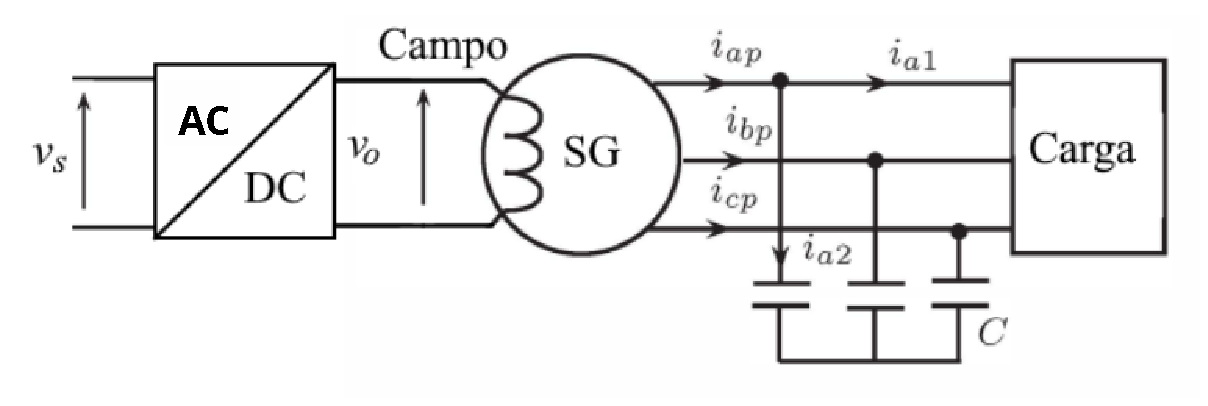
\includegraphics[width=0.5\textwidth]{Tarea_1_2}
    \end{figure}
    \begin{enumerate}[label=\alph*)]
        \item \textbf{(0.5 Puntos)} Dado el esquema visto en la figura anterior, fabrique el conversor AC/DC , para obtener una $V_{o}= 120[V]$ mediante un rectificador de onda completa monofásico. Considere que la frecuencia de la red es de $50[Hz]$ y que su condensador es de $C=1[F]$, ¿Cuál es el valor de $V_{s}$ para poder tener V0=120V?
        \item \textbf{(0.5 Puntos)} Realice el mismo procedimiento y obtenga $V_{s}$ para un rectificador de onda completa pasivo. ¿Cómo cambian sus resultados al usar un rectificador de onda completa controlado? ¿Cómo influye $\alpha$?
        \item \textbf{(2 Puntos)} Simule los tres casos y analice el comportamiento para distintos valores de C y $\alpha$. ¿Qué puede concluir con respecto al uso de los 3 rectificadores y los valores de voltaje $V_{s}$ y el tamaño de C?
        \item \textbf{(3 Puntos)} La conexión de paneles solares a la red eléctrica se hace mediante el uso de inversores de potencia. Además, para poder entregar energía cuando la disponibilidad solar es baja se utilizan sistemas de almacenamiento de energía.  Al respecto, investigue sobre distintas topologías de conexión de paneles solares con sistema de almacenamiento a la red eléctrica (describa al menos 3) y comente sobre las ventajas y desventajas de cada método. Utilice referencias en formato IEEE.
    \end{enumerate}
\end{questions}
Para la realizacion de la tarea se puede utilizar el software de simulacion que estime conveniente (\textit{Recomiendo personalmente PLECS}). Todo los graficos deben estar bien rotulados , ademas mostrar los esquemas realizados en la simulacion como los parametros utilziados.
\end{document}